
%
%   trk_performance.tex
%       author: Omar Moreno <omoreno1@ucsc.edu>
%      created: December 4, 2012
%
 
Reconstructed clusters which are in adjacent Si planes (See ...) are combined to 
form 2-dimensional ``stereo hits''.  A tracking strategy is then used by the 
tracking algorithm to form tracks using the stereo hits.  A more complete
description of the tracking algorithm can be found here [].  

The hit efficiencies were calculated for every layer using each of the available
runs. Tracks were fit using only 4 out of the 5 SVT layers and where then 
\begin{figure}[h]
    \begin{center}
        % TODO: Need to update the plot so that Layer 2 on the bottom doesn't 
        % look terrible
    	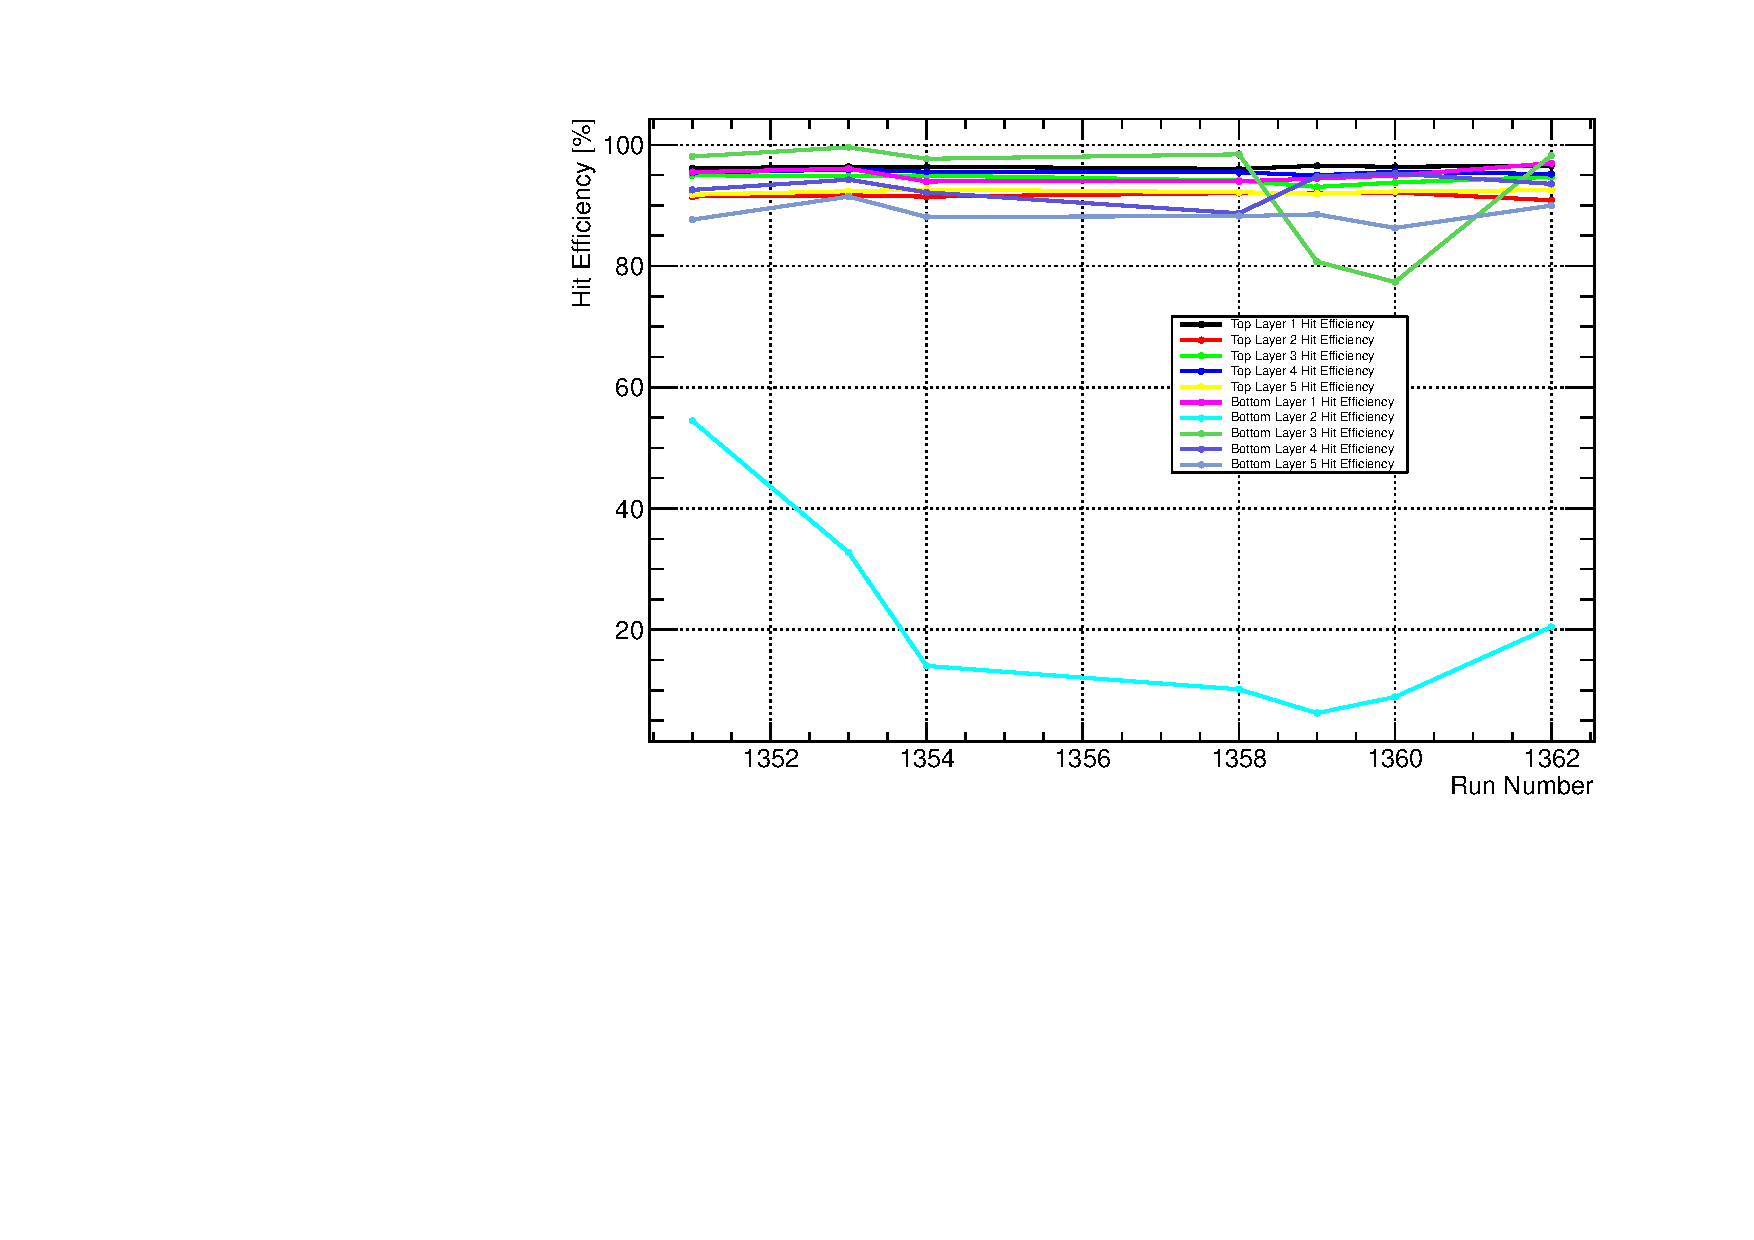
\includegraphics[width=0.98\textwidth]{test2012/svtperformance/trk_performance/hit_efficiency_vs_rn.pdf}
        \caption{} 
	\label{fig:hit_efficiency}
    \end{center}
\end{figure}
extrapolated to the layer which was not used in the fit. If the track was 
found to lie within within the layer acceptance, a stereo hit was searched
for within a window of 3 $\sigma_{\mbox{residual}}$.  The hit efficiency is
then defined as
\[
    \varepsilon_{\mbox{hit efficiency}} = \frac{\mbox{Tracks with hit on missing layer}}
                                            {\mbox{Tracks within layer acceptance}}
\]
The efficiencies of all layers, excluding all known bad modules,  was found to 
be greater then 90\%.
 
